\documentclass[tikz, border=1mm]{standalone}
\usepackage{tikz}
\usepackage{xparse}
\usetikzlibrary{calc,arrows}
% \usepackage[european]{circuitikz}
\usetikzlibrary{circuits.logic.IEC}


\makeatletter
\newcommand\currentcoordinate{\the\tikz@lastxsaved,\the\tikz@lastysaved}
\makeatother

\def\DFFsync(#1)#2{%
  \begin{scope}[shift={(#1)}]
    \node at (0.5,1.2) {$D$};
    \draw (0,0) rectangle (1,1);
    \draw (0.5,1) -- (0.5,0);
    \draw (0.5,0.5) -- (1,0.5);
    % Input
    \node at (0.75,0.75) {$Q$};
    \node at (0.75,0.25) {$\bar{Q}$};
    \draw (1,0.8) -- +(0.25,0) coordinate ({#2}Q);
    \draw (1,0.2) -- +(0.25,0) coordinate ({#2}nQ);

    % Output
    \draw (0,0.8) node[right] {$D$} -- +(-0.25,0) coordinate ({#2}D);
    \draw (0,0.2) node[right] {$C$} -- +(-0.25,0) coordinate ({#2}C);
  \end{scope}
}

\def\TFF(#1)#2{%
  \begin{scope}[shift={(#1)}]
    \node at (0.5,1.2) {$T$};
    \draw (0,0) rectangle (1,1);
    \draw (0.5,1) -- (0.5,0);
    \draw (0.5,0.5) -- (1,0.5);
    % Input
    \node at (0.75,0.75) {$Q$};
    \node at (0.75,0.25) {$\bar{Q}$};
    \draw (1,0.8) -- +(0.25,0) coordinate (#2 Q);
    \draw (1,0.2) -- +(0.25,0) coordinate (#2 nQ);
    % Output
    \draw (0,0.8) node[right] {$T$} -- +(-0.25,0) coordinate (#2 T);
    \draw (0,0.2) node[right] {$C$} -- +(-0.25,0) coordinate (#2 C);
  \end{scope}
}


\def\JKFFsync(#1)#2{%
  \begin{scope}[shift={(#1)}]
    \node at (0.5,1.8) {$JK$};
    \draw (0,0) rectangle (1,1.6);
    \draw (0.5,1.6) -- (0.5,0);
    \draw (0.5,0.8) -- (1,0.8);
% Input
    \node at (0.75,1.2) {$Q$};
    \node at (0.75,0.4) {$\bar{Q}$};
    \draw (1,1.2) -- +(0.25,0) coordinate (#2 Q);
    \draw (1,0.4) -- +(0.25,0) coordinate (#2 nQ);
% Output
    \draw (0,0.2) node[right] {$\bar{R}$} -- +(-0.25,0) coordinate (#2 nR);
    \draw (0,0.5) node[right] {$K$} -- +(-0.25,0) coordinate (#2 K);
    \draw (0,0.8) node[right] {$C$} -- +(-0.25,0) coordinate (#2 C);
    \draw (0,1.1) node[right] {$J$} -- +(-0.25,0) coordinate (#2 J);
    \draw (0,1.4) node[right] {$\bar{S}$} -- +(-0.25,0) coordinate (#2 nS);
  \end{scope}
}


\def\JKFF(#1)#2{%
  \begin{scope}[shift={(#1)}]
    \node at (0.5,1.2) {$JK$};
    \draw (0,0) rectangle (1,1);
    \draw (0.5,1) -- (0.5,0);
    \draw (0.5,0.5) -- (1,0.5);
    % Input
    \node at (0.75,0.75) {$Q$};
    \node at (0.75,0.25) {$\bar{Q}$};
    \draw (1,0.75) -- +(0.25,0) coordinate (#2 Q);
    \draw (1,0.25) -- +(0.25,0) coordinate (#2 nQ);
    % Output
    \draw (0,0.2) node[right] {$K$} -- +(-0.25,0) coordinate (#2 K);
    \draw (0,0.5) node[right] {$T$} -- +(-0.25,0) coordinate (#2 T);
    \draw (0,0.8) node[right] {$J$} -- +(-0.25,0) coordinate (#2 J);
  \end{scope}
}



\def\DEMUX1:4(#1)#2{%
  \begin{scope}[shift={(#1)}]
    \node at (0.5,2.2) {$DMUX$};
    \draw (0,0) rectangle (1,2);
    \draw (0.5,2) -- (0.5,0);
    % Output

    \draw (1,0.25) -- +(0.25,0) coordinate (#2 x3);
    \node at (0.75,0.25) {$x_3$};
    \draw (0,0.5) -- (1,0.5);

    \draw (1,0.75) -- +(0.25,0) coordinate (#2 x2);
    \node at (0.75,0.75) {$x_2$};
    \draw (0,1) -- (1,1);

    \draw (1,1.25) -- +(0.25,0) coordinate (#2 x1);
    \node at (0.75,1.25) {$x_1$};
    \draw (0,1.5) -- (1,1.5);

    \draw (1,1.75) -- +(0.25,0) coordinate (#2 x0);
    \node at (0.75,1.75) {$x_0$};

    % Input
    \draw (0,1.75) node [right] {$I$} -- +(-0.25,0) coordinate (#2 I);
    \draw (0,1.25) node [right] {$E$} -- +(-0.25,0) coordinate (#2 E);
    \draw (-0.05,0.75) node [right] {$S_0$} ++(0.05,0) -- +(-0.25,0) coordinate (#2 S0);
    \draw (-0.05,0.25) node [right] {$S_1$} ++(0.05,0) -- +(-0.25,0) coordinate (#2 S1);
  \end{scope}
}



\def\MUX4:1(#1)#2{%
  \begin{scope}[shift={(#1)}]
    \node at (0.5,3.7) {$MUX$};
    \draw (0,0) rectangle (1,3.5);
    \draw (0.5,3.5) -- (0.5,0);
    % Output
    \draw (1,1.75) -- +(0.25,0) coordinate (#2 X);
    \node at (0.75,1.75) {$X$};

    % Input
    \draw (-0.05,3.25) node [right] {$a_0$} ++(0.05,0) -- +(-0.25,0) coordinate (#2 S0);
    \draw (-0.05,2.75) node [right] {$a_1$} ++(0.05,0) -- +(-0.25,0) coordinate (#2 S1);
    \draw (-0.05,2.25) node [right] {$a_2$} ++(0.05,0) -- +(-0.25,0) coordinate (#2 S2);
    \draw (-0.05,1.75) node [right] {$a_3$} ++(0.05,0) -- +(-0.25,0) coordinate (#2 S3);


    \draw (0,1.25) node [right] {$E$} -- +(-0.25,0) coordinate (#2 E);
    \draw (-0.05,0.75) node [right] {$S_0$} ++(0.05,0) -- +(-0.25,0) coordinate (#2 S0);
    \draw (-0.05,0.25) node [right] {$S_1$} ++(0.05,0) -- +(-0.25,0) coordinate (#2 S1);
  \end{scope}
}

%#== Decoder N-2^n

\ExplSyntaxOn

\tl_new:N \l_DECDn_inports_tl

\keys_define:nn { DECDnC }
{
  innum .tl_set:N = \l_DECDn_inports_tl,
  innum .initial:n = 2,
}

\NewDocumentCommand{\DECDn}{o m m}{

  \IfNoValueF{#1}{
    \keys_set:nn { DECDnC }{ #1 }
  }

  \group_begin:

  \int_zero_new:N \l_out_ports_int
  \int_set:Nn \l_out_ports_int {\fp_to_int:n { 2 ** \l_DECDn_inports_tl }}
  \fp_zero_new:N \l_rectangle_size_fp
  \fp_set:Nn \l_rectangle_size_fp {\l_out_ports_int / 2}

  \begin{scope}[shift={(#2)}]
    \node
    (#3~center)
    at (0.75, \fp_eval:n{\l_rectangle_size_fp / 2})
    {};

    \node
    at (0.75,\fp_eval:n{\l_out_ports_int / 2 + 0.2})
    {DECD{\l_DECDn_inports_tl}:{\int_use:N \l_out_ports_int}};

    \draw (0,0) rectangle (1.5, \l_out_ports_int / 2 );

    \int_step_inline:nnn{0}{\int_use:N \l_out_ports_int - 1}{
      \draw
      (0.75,\fp_eval:n {\l_rectangle_size_fp - 0.25 - 0.5 * ##1})
      node[right] {$x\sb{##1}$}
      ++(0.75,0) -- +(0.25,0)
      coordinate (#3~x##1);
    }

    \int_step_inline:nnn{0}{\l_DECDn_inports_tl - 1}{
      \draw
      (0.65, \fp_eval:n {2 ** (\l_DECDn_inports_tl - 1) - 0.5 * ##1 - 0.25})
      node[left] {$a\sb{##1}$}
      ++(-0.65,0) -- +(-0.25,0)
      coordinate (#3~a##1);
    }

    \draw (0.6, 0.25) node[left] {$E$} ++(-0.6,0) -- +(-0.25,0) coordinate (#3~E);
  \end{scope}

  \group_end:
}


\tl_new:N \l_ENCn_inports_tl

\keys_define:nn { ENCnC }
{
  innum .tl_set:N = \l_ENCn_inports_tl,
  innum .initial:n = 2,
}

\NewDocumentCommand{\ENCn}{o m m}{

  \IfNoValueF{#1}{
    \keys_set:nn { ENCnC }{ #1 }
  }

  \group_begin:

  \int_zero_new:N \l_out_ports_int
  \int_set:Nn \l_out_ports_int {\fp_to_int:n { 2 ** \l_ENCn_inports_tl }}
  \fp_zero_new:N \l_rectangle_size_fp
  \fp_set:Nn \l_rectangle_size_fp {\l_out_ports_int / 2 + 0.5}

  \begin{scope}[shift={(#2)}]
    \node at (0.75,\fp_eval:n{\fp_use:N \l_rectangle_size_fp + 0.2})
      {ENC{\l_ENCn_inports_tl}:{\int_use:N \l_out_ports_int}};

    \draw (0,0) rectangle (1.5, \fp_use:N \l_rectangle_size_fp);

    \int_step_inline:nnn{0}{\int_use:N \l_out_ports_int - 1}{
      \draw (0.75, 0.75 + 0.5 * ##1) node[left] {$x\sb{##1}$}
      ++(0.75,0) -- +(0.25,0) coordinate (#3~x##1);
    }

    \int_step_inline:nnn{0}{\l_ENCn_inports_tl - 1}{
      \draw (0.75, \fp_eval:n {\fp_use:N \l_rectangle_size_fp - 0.5 * ##1 - 0.25})
      node[right] {$a\sb{##1}$}
      ++(-0.75,0) -- +(-0.25,0) coordinate (#3~a##1);
    }

    \draw (0.6, 0.25) node[left] {$E$} ++(-0.6,0) -- +(-0.25,0) coordinate (#3~E);
  \end{scope}

  \group_end:
}


\ExplSyntaxOff

\begin{document}

% \begin{tikzpicture}
%   \ENCn[innum=2]{0,0}{mux2}
%   \ENCn[innum=3]{2,0}{mux3}
%   \ENCn[innum=4]{4,0}{mux4}
% \end{tikzpicture}
%
% 
\begin{tikzpicture}[circuit logic IEC]
  \DECDn[innum=2]{0,0}{decd1}

  \node[or gate, inputs={nnnn}] (or) at (6,4.5) {};

  \foreach \idx in {0,1,2,3}{
    \node
    [and gate, inputs={nn}]
    (and\idx) at (4,3.2+1.2*\idx) {};

    \draw
    [very thick, red]
    (decd1 x\idx) -- ++(right:0.3+0.2*\idx) |- ({and\idx}.input 1);

    \pgfmathsetmacro{\num}{int(\idx+1)}

    \draw
    [very thick]
    ({and\idx}.output)
    -- ++(right:0.2 + 0.2*\idx)
    |- (or.input \num);

    \node
    [buffer gate, inputs={n}]
    (buffer\idx) at ({decd1 center} |- {{and\idx}.input 2}) {};

    \draw
    [very thick]
    ({buffer\idx}.output)
    |- ({and\idx}.input 2);

    \draw
    [very thick]
    ({buffer\idx}.input)
    -- ++(left:0.3);
  }

\end{tikzpicture}
% 
\begin{tikzpicture}[circuit logic IEC]
  \DECDn[innum=2]{0,0}{decd1}
  \foreach \idx in {0,1,2,3}{
    \node
    [and gate, inputs={nn}]
    (and\idx) at (4,3+1.2*\idx) {};

    \draw
    [very thick, red]
    (decd1 x\idx) -- ++(right:0.3+0.2*\idx) |- ({and\idx}.input 1);

    \node
    [buffer gate, inputs={n}]
    (buffer\idx) at ($(and\idx) + (right:1)$) {};

    \draw
    [very thick]
    ({buffer\idx}.output) -- ++(0.25,0);

    \draw
    [very thick]
    ({and\idx}.output) -- ({buffer\idx}.input);
  }

  \node [buffer gate, inputs={n}] (buffer) at (decd1 center |- or) {};

  \draw
  [very thick]
  (buffer.output)
  -- ++(right:0.4)
  coordinate (splitter);

  \foreach \idx in {0,1,2,3}{
    \draw
    [very thick]
    (splitter)
    -- ++(right:0.2 + 0.2 * \idx)
    |- ({and\idx}.input 2);
  }
\end{tikzpicture}
% 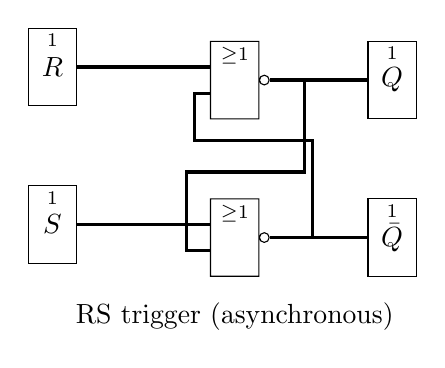
\begin{tikzpicture}[circuit logic IEC]
  \node
  [nor gate, inputs={nn}]
  (nor1) at (3,2) {};

  \node
  [nor gate, inputs={nn}]
  (nor2) at (3,0) {};

  \node
  [buffer gate, inputs={n}]
  (R) at ($(nor1.input 1) + (-2,0)$) {$R$};

  \node
  [buffer gate, inputs={n}]
  (S) at ($(nor2.input 1) + (-2,0)$) {$S$};


  \node
  [buffer gate, inputs={n}]
  (outQ) at (5,2) {$Q$};

  \node
  [buffer gate, inputs={n}]
  (outnQ) at (5,0) {$\bar{Q}$};

  \draw
  [very thick]
  (nor1.output) -- (outQ.input);

  \draw
  [very thick]
  (nor2.output) -- (outnQ.input);

  \draw
  [very thick]
  (R.output) --  (nor1.input 1);

  \draw
  [very thick]
  (S.output) --  (nor2.input 1);

  \draw
  [very thick]
  (nor1.input 2)
  -- ++ (left:0.2)
  -- ++ (down:0.6)
  -- ++ (right:1.5)
  -- (\currentcoordinate |- nor2.output);

  \draw
  [very thick]
  (nor2.input 2)
  -- ++ (left:0.3)
  -- ++ (up:1)
  -- ++ (right:1.5)
  -- (\currentcoordinate |- nor1.output);

  \node at (3,-1) {RS trigger (asynchronous)};
\end{tikzpicture}

%

\def\MUX21(#1)#2{%
  \begin{scope}[shift={(#1)}]
    \draw (0,0) rectangle (0.75,1.2);
    \draw (0,0.6) -- (0.375, 0.6);
    \draw (0.375,0) -- (0.375, 1.2);
    \node at (0.17, 0.32) {{$\&$}};
    \node at (0.17, 0.92) {{$\&$}};
    \node at (0.55, 0.6) {$1$};

    \draw[very thick] (0.75, 0.6)
    -- ++(right:0.25)
    coordinate ({#2}out);

    \draw[very thick] (0, 0.2)
    -- ++(left:0.25)
    coordinate ({#2}in1);

    \draw[very thick] (0, 0.4)
    -- ++(left:0.25)
    coordinate ({#2}en1);

    \draw[very thick] (0, 0.7)
    -- ++(left:0.25)
    coordinate ({#2}in2);

    \draw[very thick] (0, 0.9)
    -- ++(left:0.25)
    coordinate ({#2}en2);
  \end{scope}
}

\begin{tikzpicture}[circuit logic IEC]
  \node
  [buffer gate, inputs={n}]
  (inClock) at (2,6.5) {$C$};

  \node
  [buffer gate, inputs={n}]
  (modeSelector) at (2,5) {$E$};

  \def\spacing{6}
  \def\initoffset{4.5}
  \def\lastindex{3}

  \foreach \idx in {0,1,...,\lastindex}{
    \node
    [buffer gate, inputs={n}]
    (inD\idx) at (2,3-\idx*1.2) {$D_{\idx}$};

    \DFFsync(\initoffset+2+\idx*\spacing,7){Dff\idx};

    \MUX21(\initoffset+\idx*\spacing,8){MUX\idx};

    %#== Input selector to trigger
    \draw
    [very thick]
    ({MUX\idx}out)
    -- ++ (right:0.1)
    |- ({Dff\idx}D);

    %#== Input selector chooser
    \draw
    [very thick, black!40!green]
    (modeSelector.output)
    -- ++($(\idx*\spacing+0.5,0)$)
    |- ({MUX\idx}en1);

    \node
    [not gate, inputs={n}]
    (not\idx) at ($(modeSelector.output) + (\idx*\spacing+1,4.3)$) {};

    \draw
    [very thick, black!60!green]
    ({not\idx}.output)
    -- ++(right:0.1)
    |- ({MUX\idx}en2);

    \draw
    [very thick, black!60!green]
    (modeSelector.output)
    -- ++($(\idx*\spacing+0.5,0)$)
    |- ({not\idx}.input);

    %#== Clock
    \draw
    [very thick, gray, densely dash dot]
    (inClock.output)
    -- ++ (right:{\idx*\spacing + 1.5})
    |- ({Dff\idx}C);

    %#== Parallel input
    \draw
    [very thick, blue]
    ({inD\idx}.output)
    -- ++($(\idx*\spacing + 0.25, 0)$)
    |- ({MUX\idx}in2);

  }

  \foreach \idx in {1,2,...,\lastindex}{
    %#== Trigger connection
    \pgfmathsetmacro{\num}{int(\idx-1)}
    \draw
    [very thick, gray]
    ({Dff\num}Q)
    --  ++(right:0.25)
    |- ({MUX\idx}in1);
  }


\end{tikzpicture}


\end{document}
